\documentclass{beamer}
\usetheme{metropolis}
\usepackage{hyperref}
\usepackage[utf8]{inputenc} % this is needed for german umlauts
\usepackage[english]{babel} % this is needed for german umlauts
\usepackage[T1]{fontenc}    % this is needed for correct output of umlauts in pdf
\usepackage{caption}
\usepackage{tikz}
\usetikzlibrary{arrows.meta}
\usetikzlibrary{decorations.pathreplacing}
\usetikzlibrary{positioning}
\usetikzlibrary{decorations.text}
\usetikzlibrary{decorations.pathmorphing}
\usetikzlibrary{shapes.multipart, calc}
\usepackage{minted} % needed for the inclusion of source code

\begin{document}

\title{Convolutional Neural Networks (CNNs)}
\subtitle{Theory and Applications}
\author{Martin Thoma}
\date{22. February 2019}
\subject{Machine Learning, AI, Neural Networks, Convolutional Neural Networks}

\frame{\titlepage}

% \section{Neural Network Basics}
% \subsection{}
\begin{frame}{Artificial Neuron (Perceptron)}
    $$f: \mathbb{R}^n \rightarrow \mathbb{R}$$
    \begin{figure}[ht]
        \centering
        \includegraphics[width=0.8\paperwidth, height=0.7\paperheight, keepaspectratio]{graphics/artificial-neuron.pdf}
    \end{figure}
    % $$f(x) = ax^2 + bx + c \text{ with } f(0) = 3, f(1) = 2, f(-1) = 6$$
    % \begin{align*}
    %     \onslide<2->{f(0) &= a \cdot 0^2 + b \cdot 0 + c = 3} &\onslide<3->{\Rightarrow c &= 3\\}
    %     \onslide<4->{f(1) &= a \cdot 1^2 + b \cdot 1 + 3 = 2} &\onslide<5->{\Rightarrow a &= -1-b\\}
    %     \onslide<6->{f(-1) &= a \cdot {(-1)}^2 - b + 3 = 6\\}
    %     \onslide<7->{\Leftrightarrow 3&=a - b\\}
    %     \onslide<8->{\Leftrightarrow 3&= (-1-b) - b\\}
    %     \onslide<9->{\Leftrightarrow b&= -2\\}
    %     \onslide<10>{\Rightarrow \quad f(x) &= x^2 -2 x + 3\\}
    % \end{align*}
%     \only<1>{$$f: \mathbb{R}^n \rightarrow \mathbb{R}^m$$}
%     \only<2>{$$f: \mathbb{R}^2 \rightarrow \mathbb{R}$$
% # 2x - 1
% # (x-1)^2 + 1
%     Examples:
%         \begin{itemize}
%             \item $1 \rightarrow 1$: $f(x) = x$
%             \item $2 \rightarrow 3$: $f(x) = $
%             % \item $3 \rightarrow 3$
%         \end{itemize}
%     }
\end{frame}

\begin{frame}{Multi-Layer Perceptron (MLP)}
    $$f: \mathbb{R}^n \rightarrow \mathbb{R}^m$$
    \begin{figure}[ht]
        \centering
        
\includegraphics[width=0.8\paperwidth, height=0.7\paperheight, keepaspectratio]{graphics/perceptron-notation.pdf}
    \end{figure}
\end{frame}

\begin{frame}{}
    \begin{itemize}[<+->]
        \item Predict housing prices: (bed rooms, size, age) $\rightarrow$ Price
        \item Product categorization: (weight, volume, price) $\rightarrow$ \{shoe, handbag, shirt\}
        \item Image classification: List of pixel colors $\rightarrow$ \{cat, dog\}
    \end{itemize}
\end{frame}

\begin{frame}{}
    \begin{center}
    \Huge Data
    \end{center}
\end{frame}

\begin{frame}{Necessary Data}
    \begin{itemize}
        \item $f(x) = w_0$
        \item $f(x) = w_1 \cdot x + w_0$
        \item $f(x) = w_2^2 \cdot x^2 + w_1^2 \cdot x + w_0$
        \item sin, cos, tan, \dots
    \end{itemize}
\end{frame}

\begin{frame}{Convolution}
\begin{figure}[ht]
    \centering
    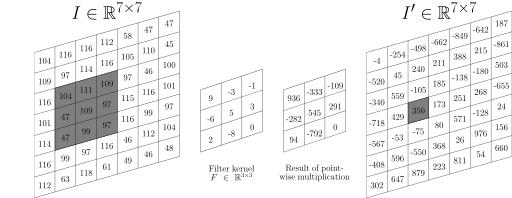
\includegraphics[width=0.8\paperwidth]{graphics/convolution-linear.pdf}
\end{figure}
\end{frame}

\begin{frame}{Convolutional Layer}
\begin{figure}[ht]
    \centering
    \documentclass{standalone}
\usepackage{amssymb}
\usepackage{tikz}
\usetikzlibrary{arrows.meta}
\usetikzlibrary{decorations.pathreplacing}

\begin{document}
\newcommand{\distance}{6}
\newcommand{\xup}{3.5}
\newcommand{\yup}{6}
\newcommand{\upsizex}{1}
\newcommand{\upsizey}{2}
\newcommand{\upshift}{3/4*\upsizey}
\newcommand{\distancedots}{1}

\begin{tikzpicture}
    % Print input feature maps
    \foreach \i in {0, 0.2, ..., 0.6} {
        \draw[fill=white] (0+\i, 0) -- (2+\i, 3) -- (2+\i, 7) -- (\i, 4) -- (\i, 0);
    }

    % Print filters
    \foreach \i in {0, 0.2, ..., 0.6, 1.3} {
        \draw[fill=white] (\xup+\i, \yup) -- (\xup+\upsizex+\i, \yup+\upshift) -- (\xup+\upsizex+\i, \yup+\upsizey+\upshift) -- (\xup+\i, \yup+\upsizey) -- (\xup+\i, \yup);
        \draw[fill=white] (\xup+\i, \yup) -- (\xup+\i+0.1, \yup) -- (\xup+\i+0.1, \yup+\upsizey) -- (\xup+\i, \yup+\upsizey) -- (\xup+\i, \yup);
        \draw[fill=white] (\xup+\i+0.1, \yup) -- (\xup+\upsizex+\i+0.1, \yup+\upshift) -- (\xup+\upsizex+\i+0.1, \yup+\upsizey+\upshift) -- (\xup+\i+0.1, \yup+\upsizey) -- (\xup+\i+0.1, \yup);
        \draw[fill=white] (\xup+\i, \yup+\upsizey) -- (\xup+\i+0.1, \yup+\upsizey) -- (\xup+\upsizex+\i+0.1, \yup+\upsizey+\upshift) -- (\xup+\upsizex+\i, \yup+\upsizey+\upshift) -- (\xup+\i, \yup+\upsizey);
    }

    \foreach \i in {0, 0.2, ..., 0.6, 1.2} {
        \draw[fill=white] (\distance+\i, 0) -- (\distance+2+\i, 3) -- (\distance+2+\i, 7) -- (\distance+\i, 4) -- (\distance+\i, 0);
    }

    \draw [decorate,decoration={brace,amplitude=+4pt,mirror},xshift=0pt,yshift=-2pt]
(-0.1,0) -- (0.7,0) node [black,midway,yshift=-0.6cm, align=center] {\footnotesize$3$ feature maps\\\footnotesize(e.g. RGB)};
    \draw [decorate,decoration={brace,amplitude=+4pt,mirror},xshift=0pt,yshift=-2pt]
(\distance-0.1,0) -- (\distance+1.3,0) node [black,midway,yshift=-0.6cm, align=center] {\footnotesize$n$ feature maps};
    \draw [decorate,decoration={brace,amplitude=+4pt},xshift=0pt,yshift=+2pt]
(\xup-0.1+\upsizex,\yup+\upsizey+\upshift) -- (\xup+1.5+\upsizex,\yup+\upsizey+\upshift) node [black,midway,yshift=+0.6cm, align=center] {\footnotesize $n$ filters of\\\footnotesize size $3\times 3 \times 3$};
    \draw[very thick, ->,>=latex] (3, 4.5) [out=70, in=110] to  (\distance-0.5, 4.5);
    \draw [color=white,decorate,decoration={brace,amplitude=+4pt, mirror},xshift=0pt,yshift=+2pt]
(1.1, 0) -- (3.1, 3) node [sloped,black,midway,yshift=+0.6cm, align=center] {width $w$};
    \draw [color=white,decorate,decoration={brace,amplitude=+4pt, mirror},xshift=0pt,yshift=+2pt]
(\distance+1.7, 0) -- (\distance+3.7, 3) node [sloped,black,midway,yshift=+0.6cm, align=center] {width $w$};
    \draw [decorate,decoration={brace,amplitude=+4pt},xshift=-2pt,yshift=0pt]
(0, 0) -- (0, 4) node [sloped,black,midway,yshift=+0.6cm, align=center] {height $h$};
    \draw [decorate,decoration={brace,amplitude=+4pt},xshift=-2pt,yshift=0pt]
(\distance, 0) -- (\distance, 4) node [sloped,black,midway,yshift=+0.6cm, align=center] {height $h$};
    \node at (-2.5,7) {\Large network};
    \node at (-2.5,2) {\Large data};
    \node at (\distance+0.95,3.9) {\dots};
    \node at (\distance+0.95,2) {\dots};
    \node at (\distance+0.95,0.1) {\dots};

    \node at (\xup+1.05,\yup+1.9) {\dots};
    \node at (\xup+1.05,\yup+1.0) {\dots};
    \node at (\xup+1.05,\yup+0.1) {\dots};
\end{tikzpicture}
\end{document}

\end{figure}
\end{frame}

\begin{frame}{Max Pooling}
\begin{figure}[ht]
    \centering
    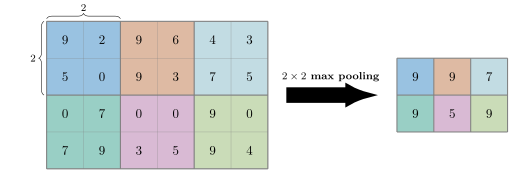
\includegraphics[width=0.8\paperwidth]{graphics/max-pooling.pdf}
\end{figure}
\end{frame}

\section{Applications}
\begin{frame}{Symbol recognizer}
\begin{figure}[ht]
    \centering
    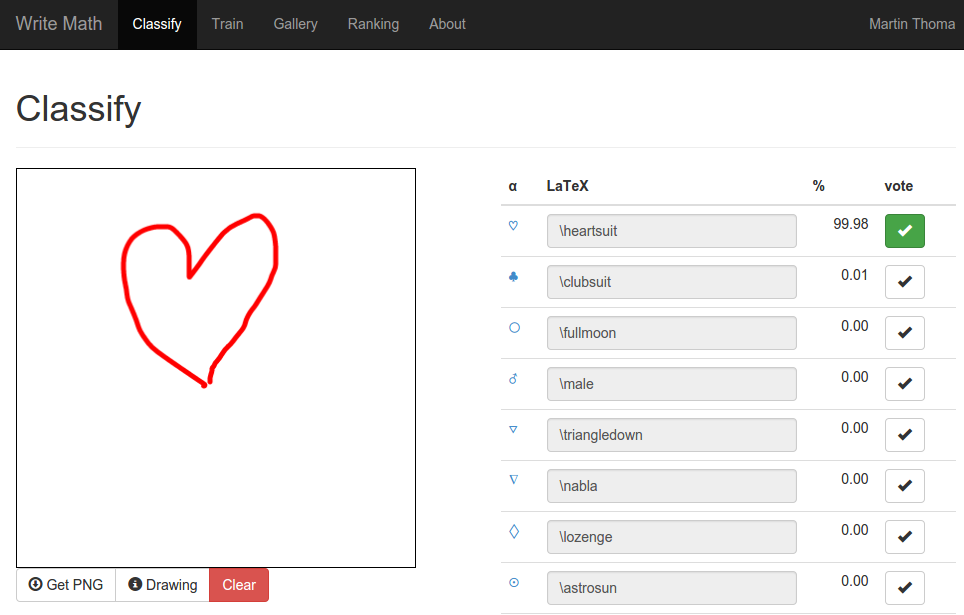
\includegraphics[width=0.8\paperwidth, height=0.7\paperheight, keepaspectratio]{graphics/symbol-recognizer.png}
    \captionsetup{labelformat=empty}
    \caption{\href{http://write-math.com}{write-math.com}}
\end{figure}
\end{frame}

\begin{frame}{}
\inputminted[linenos,
               numbersep=7pt,
               gobble=0,
               % frame=none,
               % framesep=2mm,
                fontsize=\footnotesize, tabsize=4]{python}{cnn.py}
\end{frame}

\begin{frame}{Super Resolution}
\begin{figure}[ht]
    \centering
    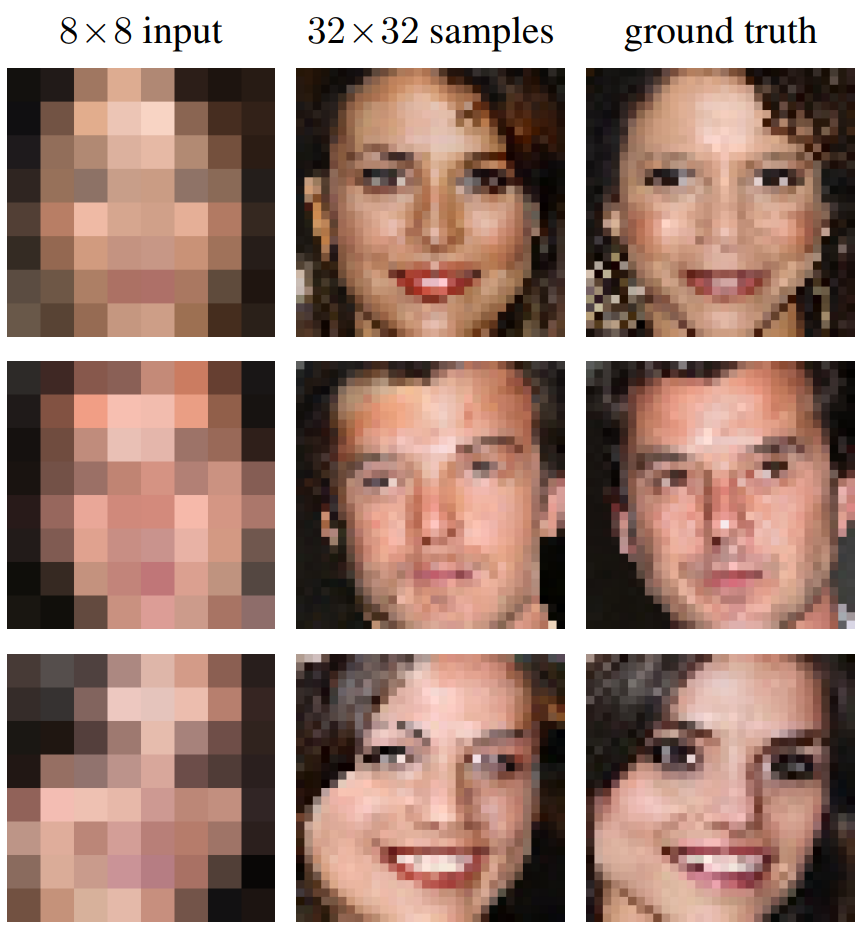
\includegraphics[width=0.8\paperwidth, height=0.7\paperheight, keepaspectratio]{graphics/pixel-recursive-super-resolution.png}
    \captionsetup{labelformat=empty}
    \caption{Dahl, Norouzi, Shlens: Pixel recursive super resolution (2017)}
\end{figure}
\end{frame}


\begin{frame}{Colorization: The Problem}
\begin{figure}[ht]
    \centering
    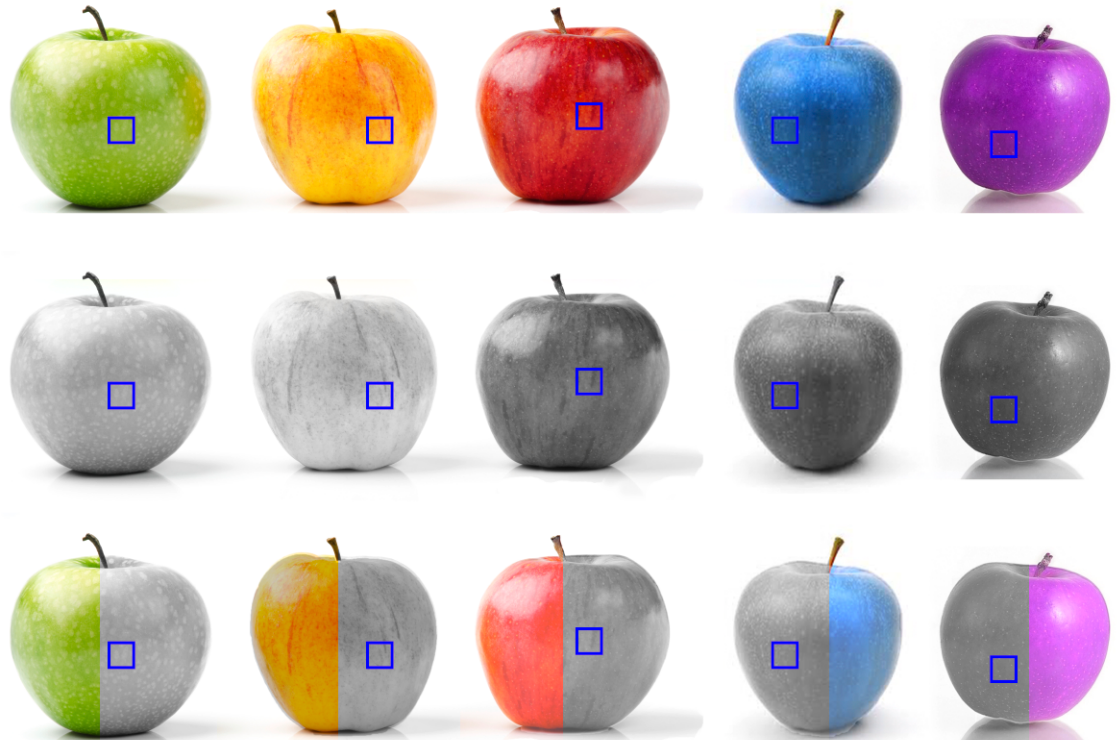
\includegraphics[width=0.8\paperwidth, height=0.7\paperheight, keepaspectratio]{graphics/multimodality-apple.png}
    \captionsetup{labelformat=empty}
    \caption{Cinarel: Automatic Colorization of Webtoons Using Deep Convolutional Neural Networks (2018)}
\end{figure}

Interactive Demo: \href{http://richzhang.github.io/colorization/}{richzhang.github.io/colorization}
\end{frame}


\begin{frame}{Colorization - Photographs}
\begin{figure}[ht]
    \centering
    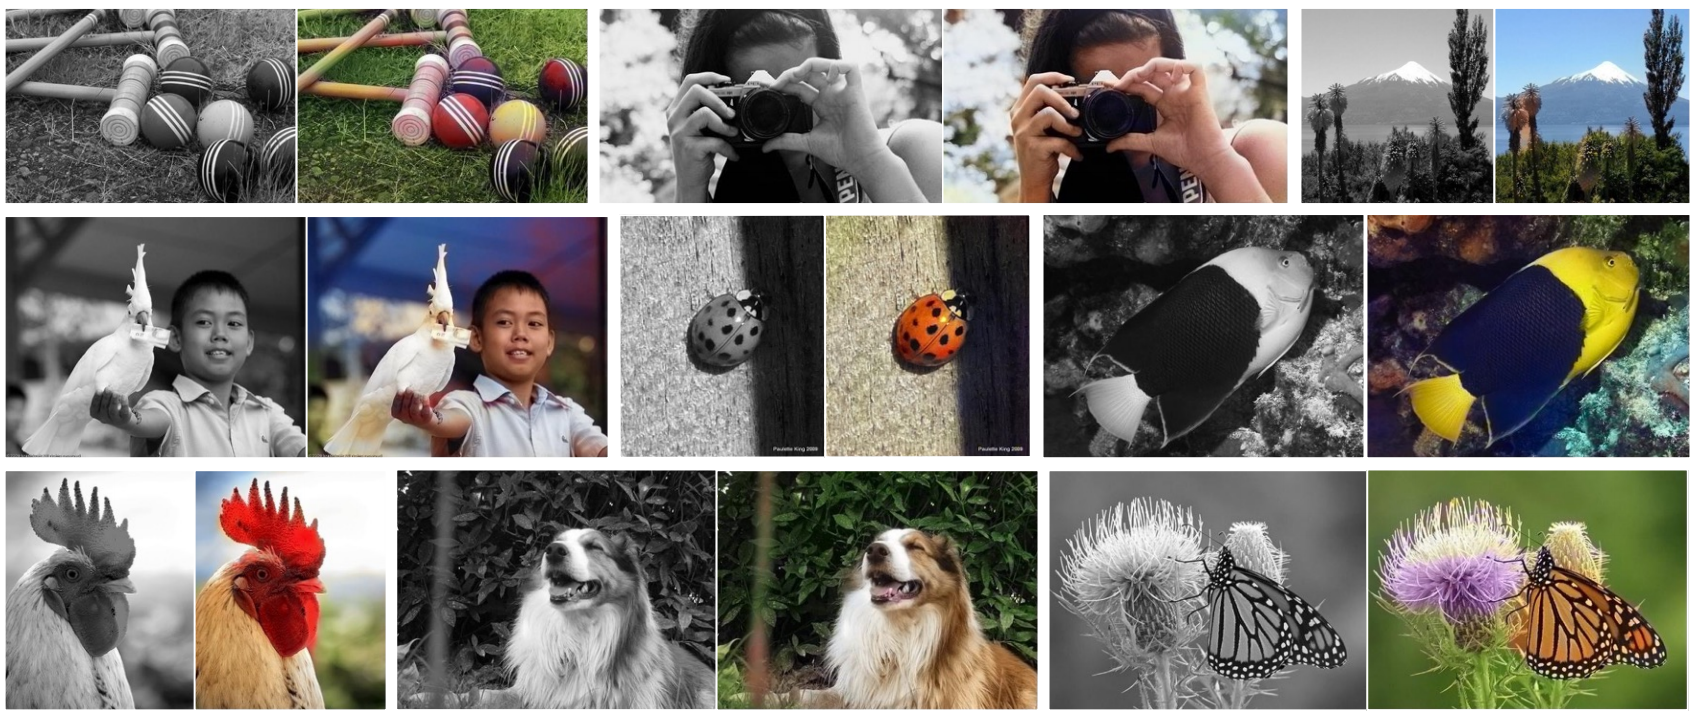
\includegraphics[width=0.8\paperwidth, height=0.7\paperheight, keepaspectratio]{graphics/colorful-image-colorization.png}
    \captionsetup{labelformat=empty}
    \caption{Zhang, Isola, Efros: Colorful Image Colorization (2016)}
\end{figure}

Interactive Demo: \href{http://richzhang.github.io/colorization/}{richzhang.github.io/colorization}
\end{frame}


\begin{frame}{Colorization - Comic}
\begin{figure}[ht]
    \centering
    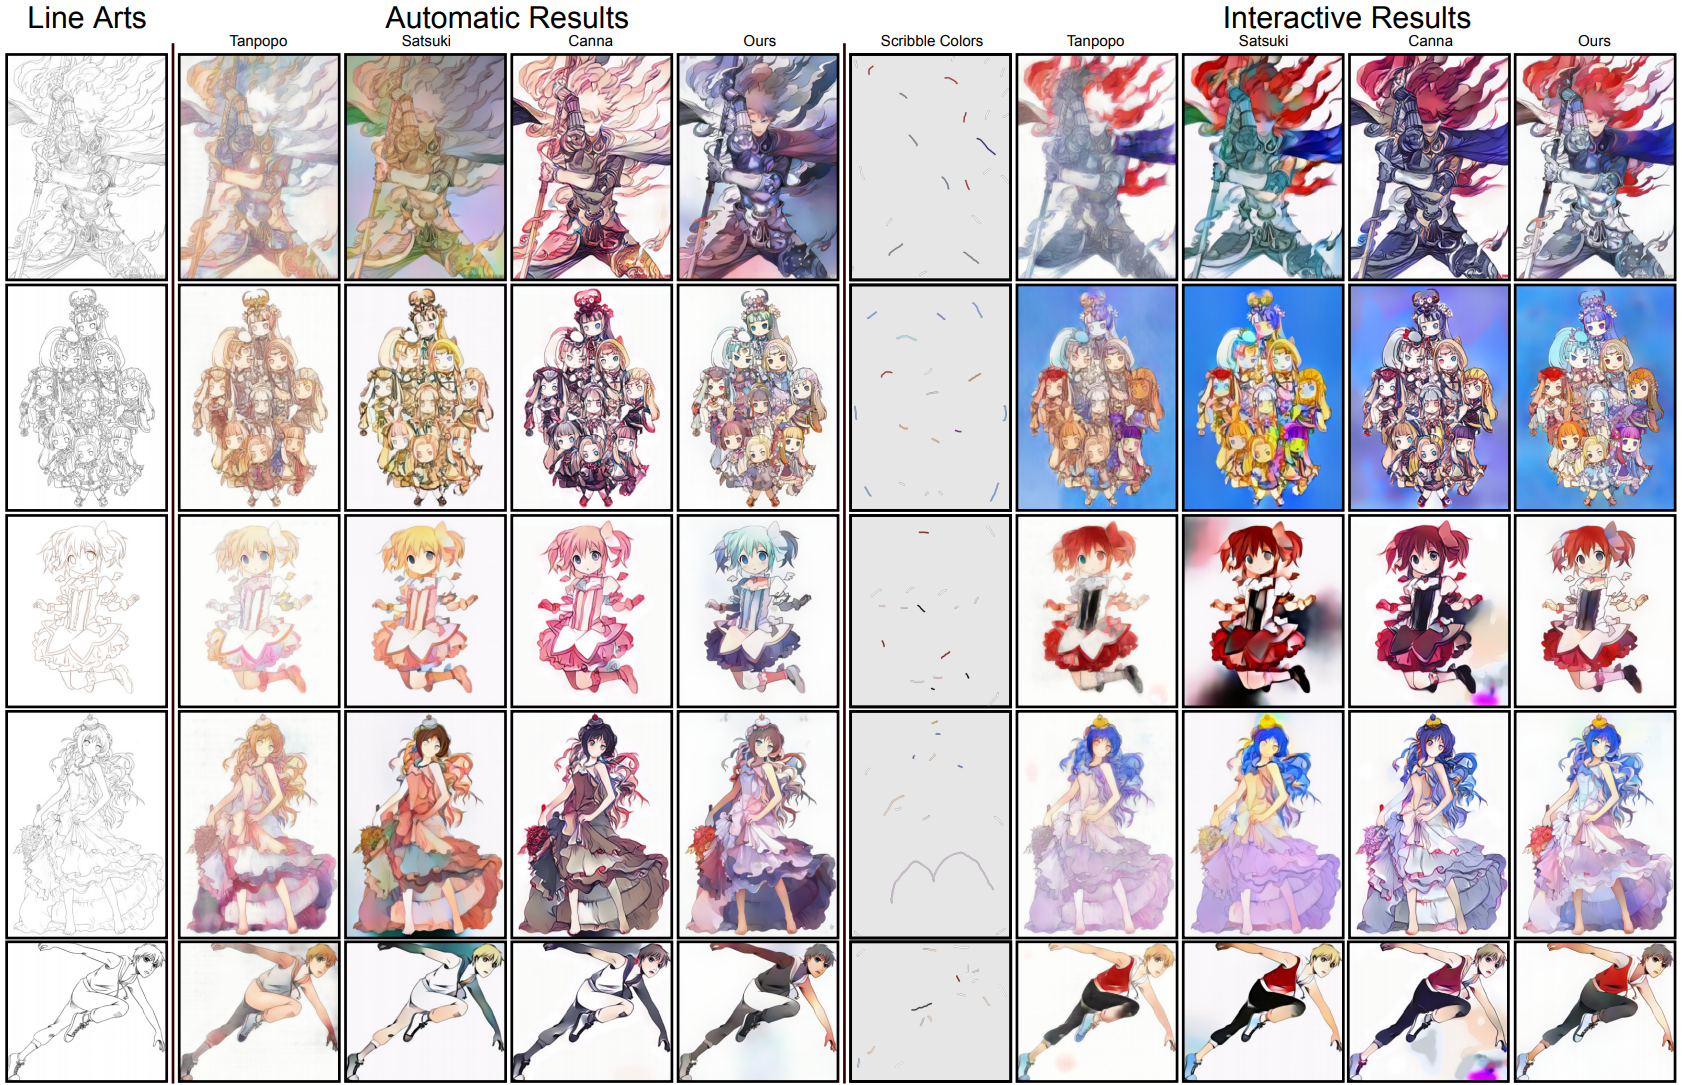
\includegraphics[width=0.8\paperwidth, height=0.7\paperheight, keepaspectratio]{graphics/comic-colorization.png}
    \captionsetup{labelformat=empty}
    \caption{Ci, Ma, Wang, Li, Luo: User-Guided Deep Anime Line Art Colorization with Conditional Adversarial Networks (2018)}
\end{figure}
\end{frame}

\begin{frame}{Denoising}
\begin{figure}[ht]
    \centering
    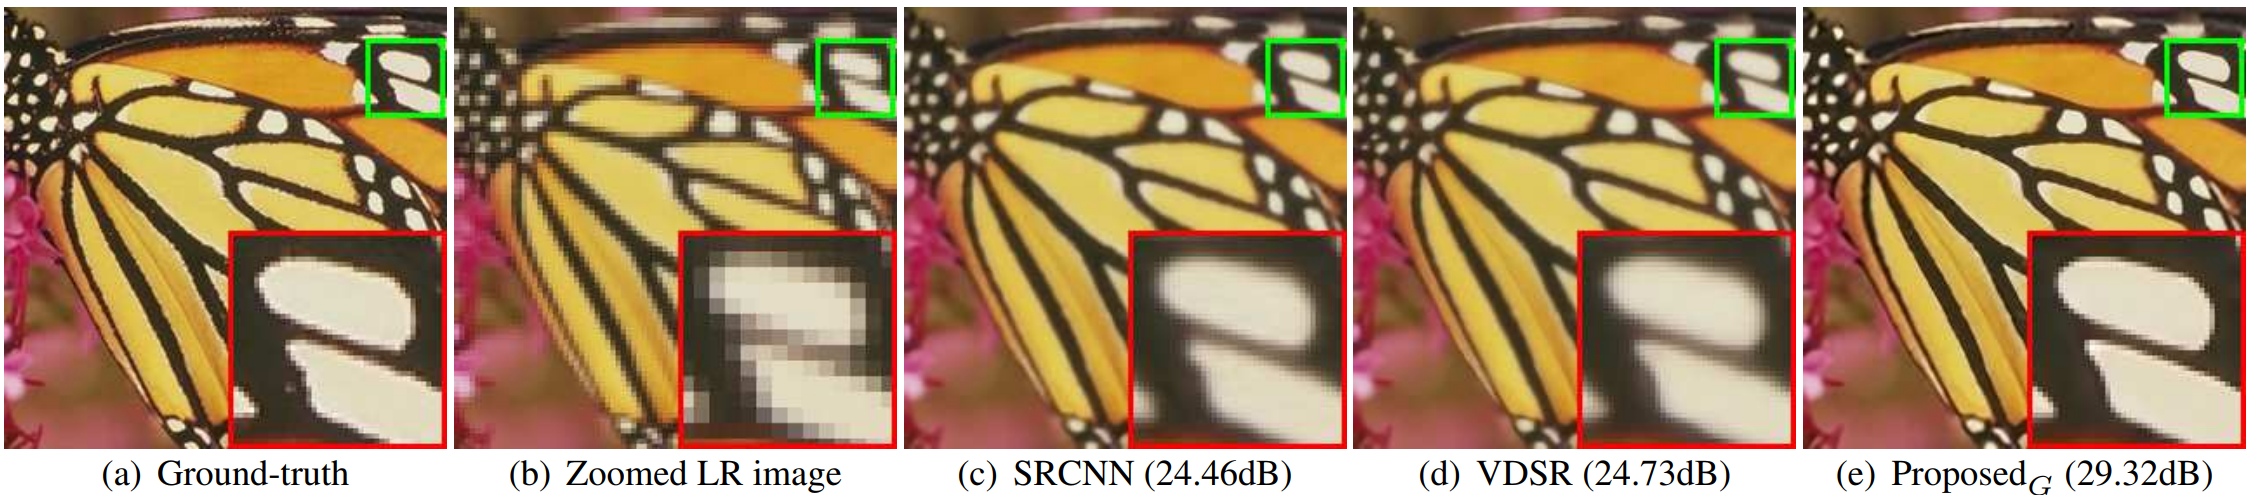
\includegraphics[width=0.8\paperwidth, height=0.7\paperheight, keepaspectratio]{graphics/denoising.png}
    \captionsetup{labelformat=empty}
    \caption{Zhang, Zuo, Gu, Zhang: Learning Deep CNN Denoiser Prior for Image Restoration (2017)}
\end{figure}
\end{frame}


\begin{frame}{Image Inpainting (Watermark removal)}
\begin{figure}[ht]
    \centering
    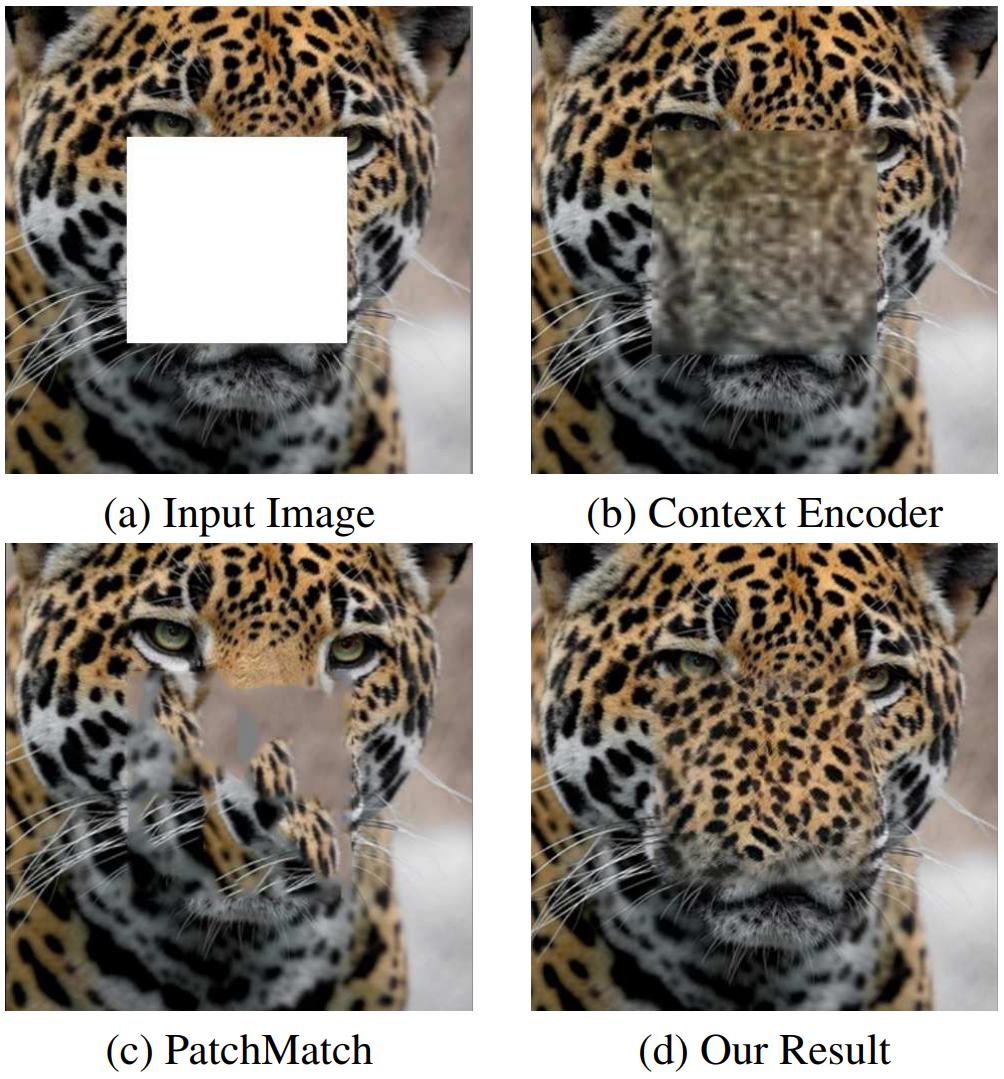
\includegraphics[width=0.8\paperwidth, height=0.7\paperheight, keepaspectratio]{graphics/leopard-inpainting.png}
    \captionsetup{labelformat=empty}
    \caption{Yang, Lu, Lin, Shechtman, Wang, Li: High-Resolution Image Inpainting using Multi-Scale Neural Patch Synthesis (2017)}
\end{figure}
\end{frame}


\begin{frame}{CNNs in NLP}
\begin{figure}[ht]
    \centering
    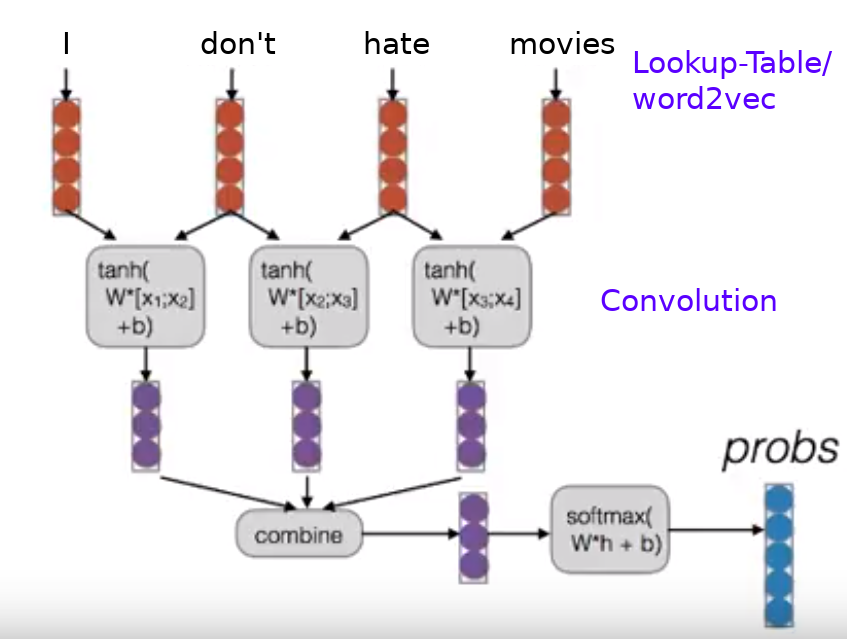
\includegraphics[width=0.8\paperwidth, height=0.7\paperheight, keepaspectratio]{graphics/tdnns.png}
    \captionsetup{labelformat=empty}
    \caption{Collobert, Weston, Bottou, Karlen, Kavukcuoglu, Kuksa: 
Natural Language Processing (almost) from Scratch (2011)}
\end{figure}
\end{frame}

\end{document}
